\documentclass{article}

\usepackage{graphicx}
\usepackage{hyperref}

\title{jettl \\ S.O.L.I.D LabVIEW Asynchronous Framework}
\author{Nathan Davis}
\date{\today}

\begin{document}

\maketitle

\maketitle

\section{Introduction}
\label{sec:introduction}

Strictly interface composition based asynchronous actor oriented design pattern for LabVIEW Applications.
jettl also has the newer banners for vis. Easy adoption for the new age of LV developers.
State pattern with decorators.
It is interface composition, so stick with the same rule set for naming methods

\section{LabVIEW Interfaces}
\label{sec:labview-interfaces}

The default implementation idea works so only as there is only one method implementation across all interfaces.

For example, \\
class implements interface 1 and interface 2 \\
interface 1: method \\
interface 2: method \\
This cannot exist unless the class overrides the method.
Otherwise, at runtime, LabVIEW does not know to execute interface 1: method or interface 2: method.

\section{Future Scope}
\label{sec:future-scope}

Creating an actor is NOT connected to the actor that creates it.
Rather, this actor exists on its own in the “liquid” message transport.
The overall “application” has access to the actor's reference (unique message address)

\subsection{Pub-Sub Messaging}
\label{subsec:pub-sub-messaging}

\begin{figure}[!ht]
    \centering
    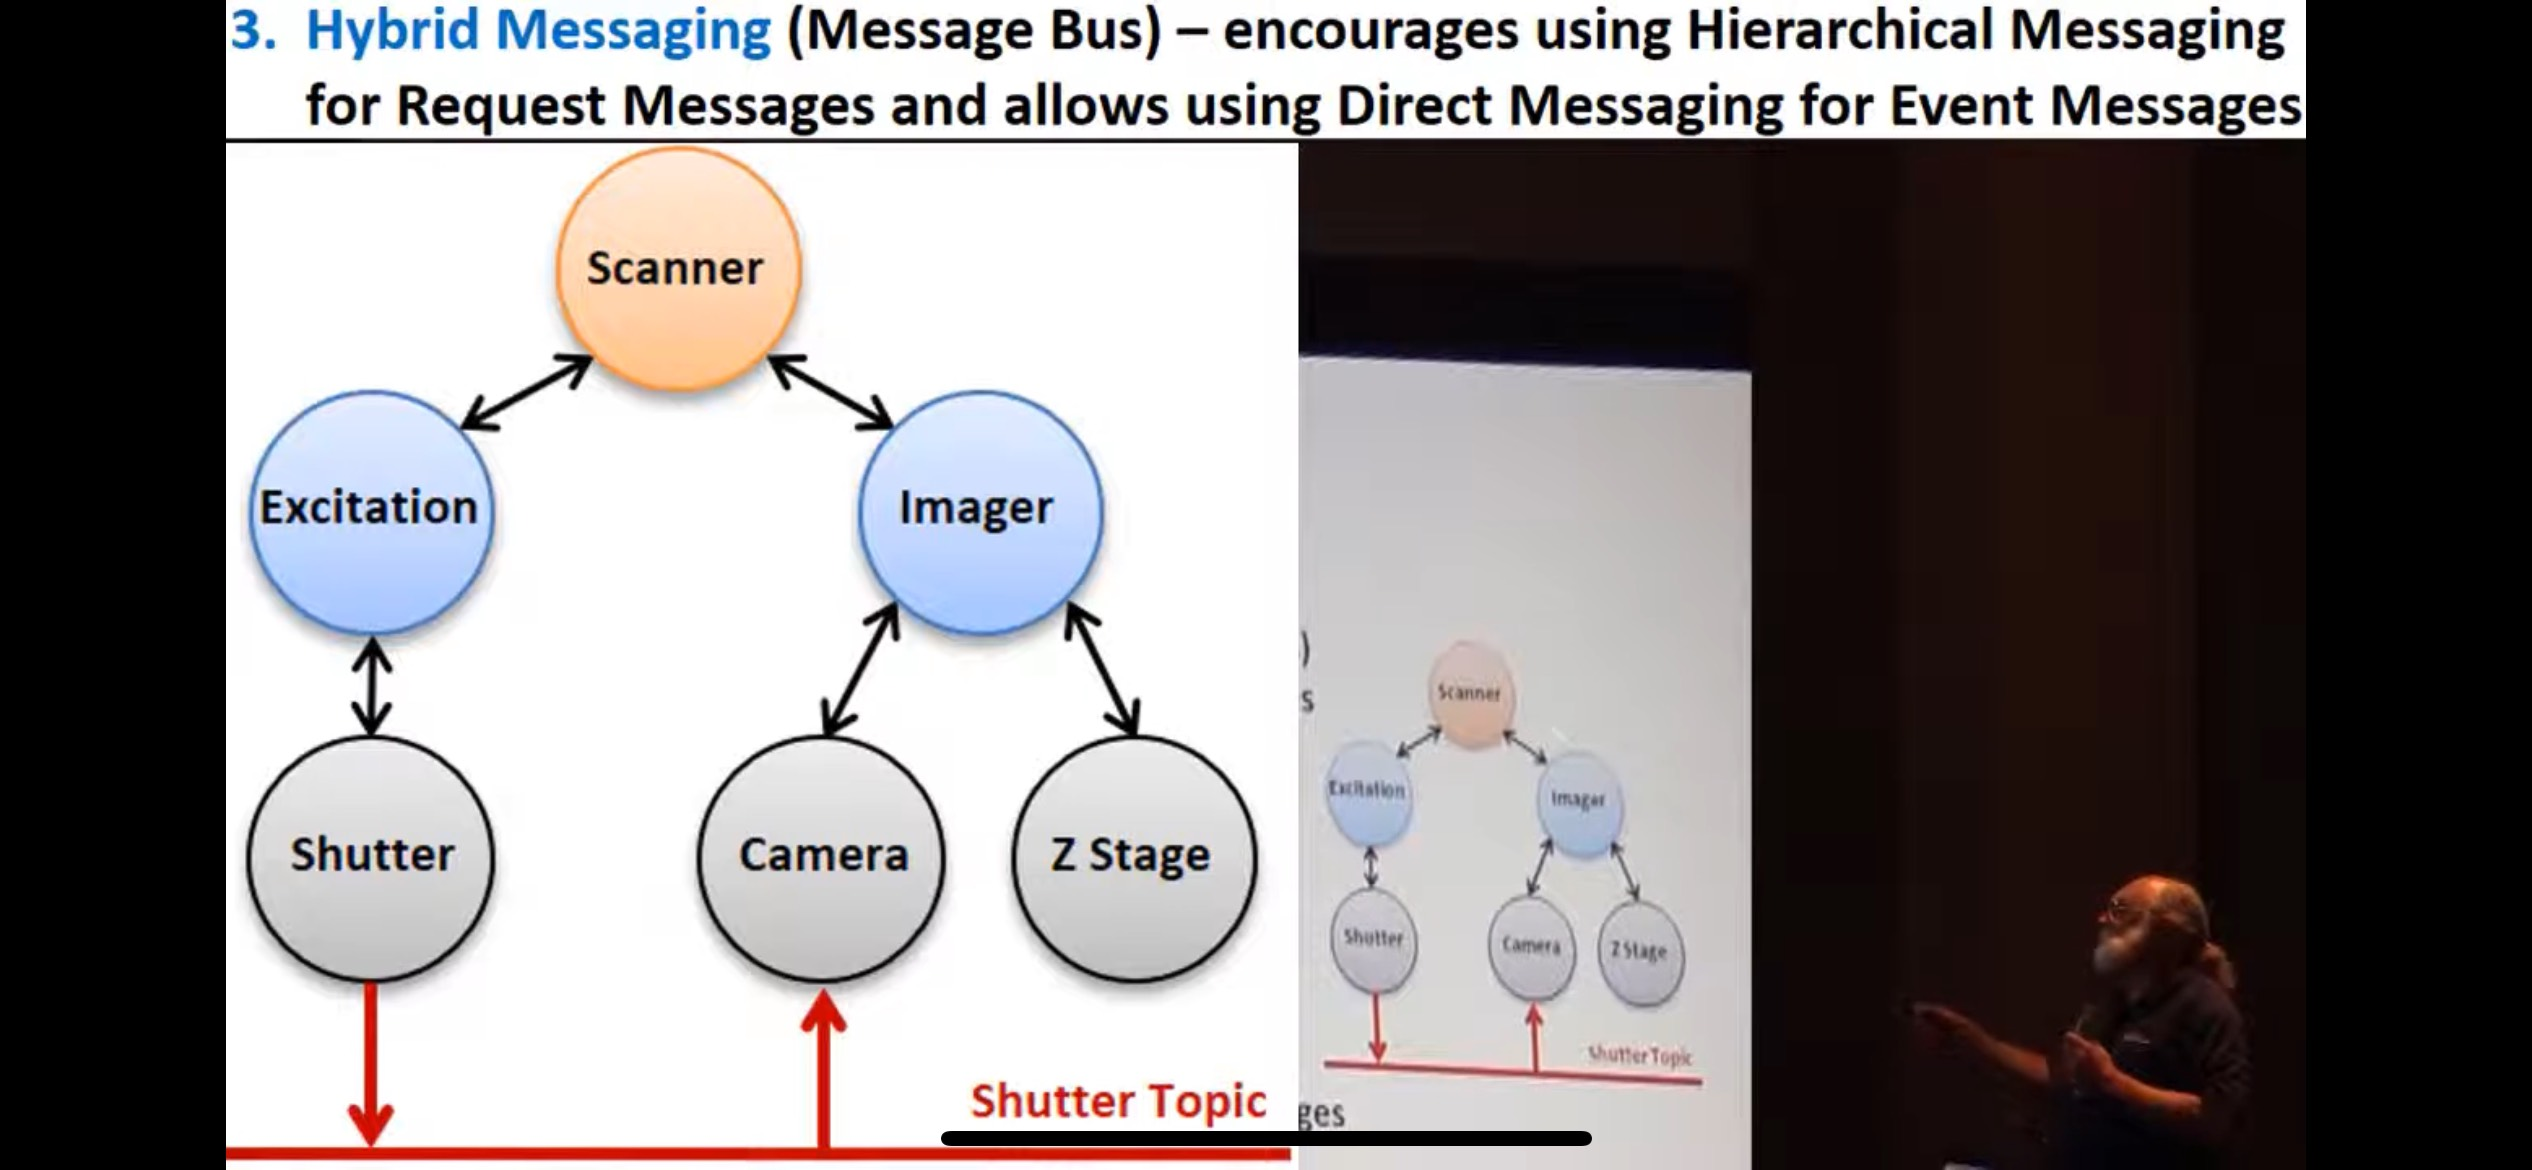
\includegraphics[width=0.8\textwidth]{figures/labview_dmitry_message _transport}
    \caption{LabVIEW Actor Framework Message Transport.}
    \label{fig:message-transport}
\end{figure}

As shown in Fig~\ref{fig:message-transport}, it is as though the actors are just objects that “float” in this “liquid” messaging transport.
So that way you can perform this pub-sub messaging.
The objects are linked together by “who launches who”.

Same as with the pub-sub pattern, everything is a publisher-subscriber.
It's just that most relationships are just one way.
Same with Git, the philosophy is that all branches are created equal

\section{Debugging}
\label{sec:debugging}

What a log for which methods are executed, instead of the dialog popups

Take out error handling for the backend, for now.
Not necessary since on the basis that the framework will not generate errors.
This may not be true in production, but for simplicity of understanding the framework, this is it.


\section{Git}
\label{sec:git}

This might be of interest for submodules in git for LabVIEW.
Find here: \href{https://www.youtube.com/watch?v=iv7WwDgyb0U}{Git Submodules: An Alternative Approach to Code Reuse - Greg Payne - GDevCon2}.

In the repos, use the tag to have different "stable" versions of the repo such as v0.1.1 or v3.8.3
This allows others to easily look at the different versions of the repo without much thought.
This could also help with submodules that are referenced in other repos.
Check this video near the end for reference: \href{https://www.youtube.com/watch?v=tRZGeaHPoaw&list=PLvDxiIkwuMQs0Uu6AIhTGqXahndMmfUyx&index=19}{Git and GitHub Tutorial for Beginners}

\section{Naming Conventions}
\label{sec:naming-conventions}

\begin{figure}[!ht]
    \centering
    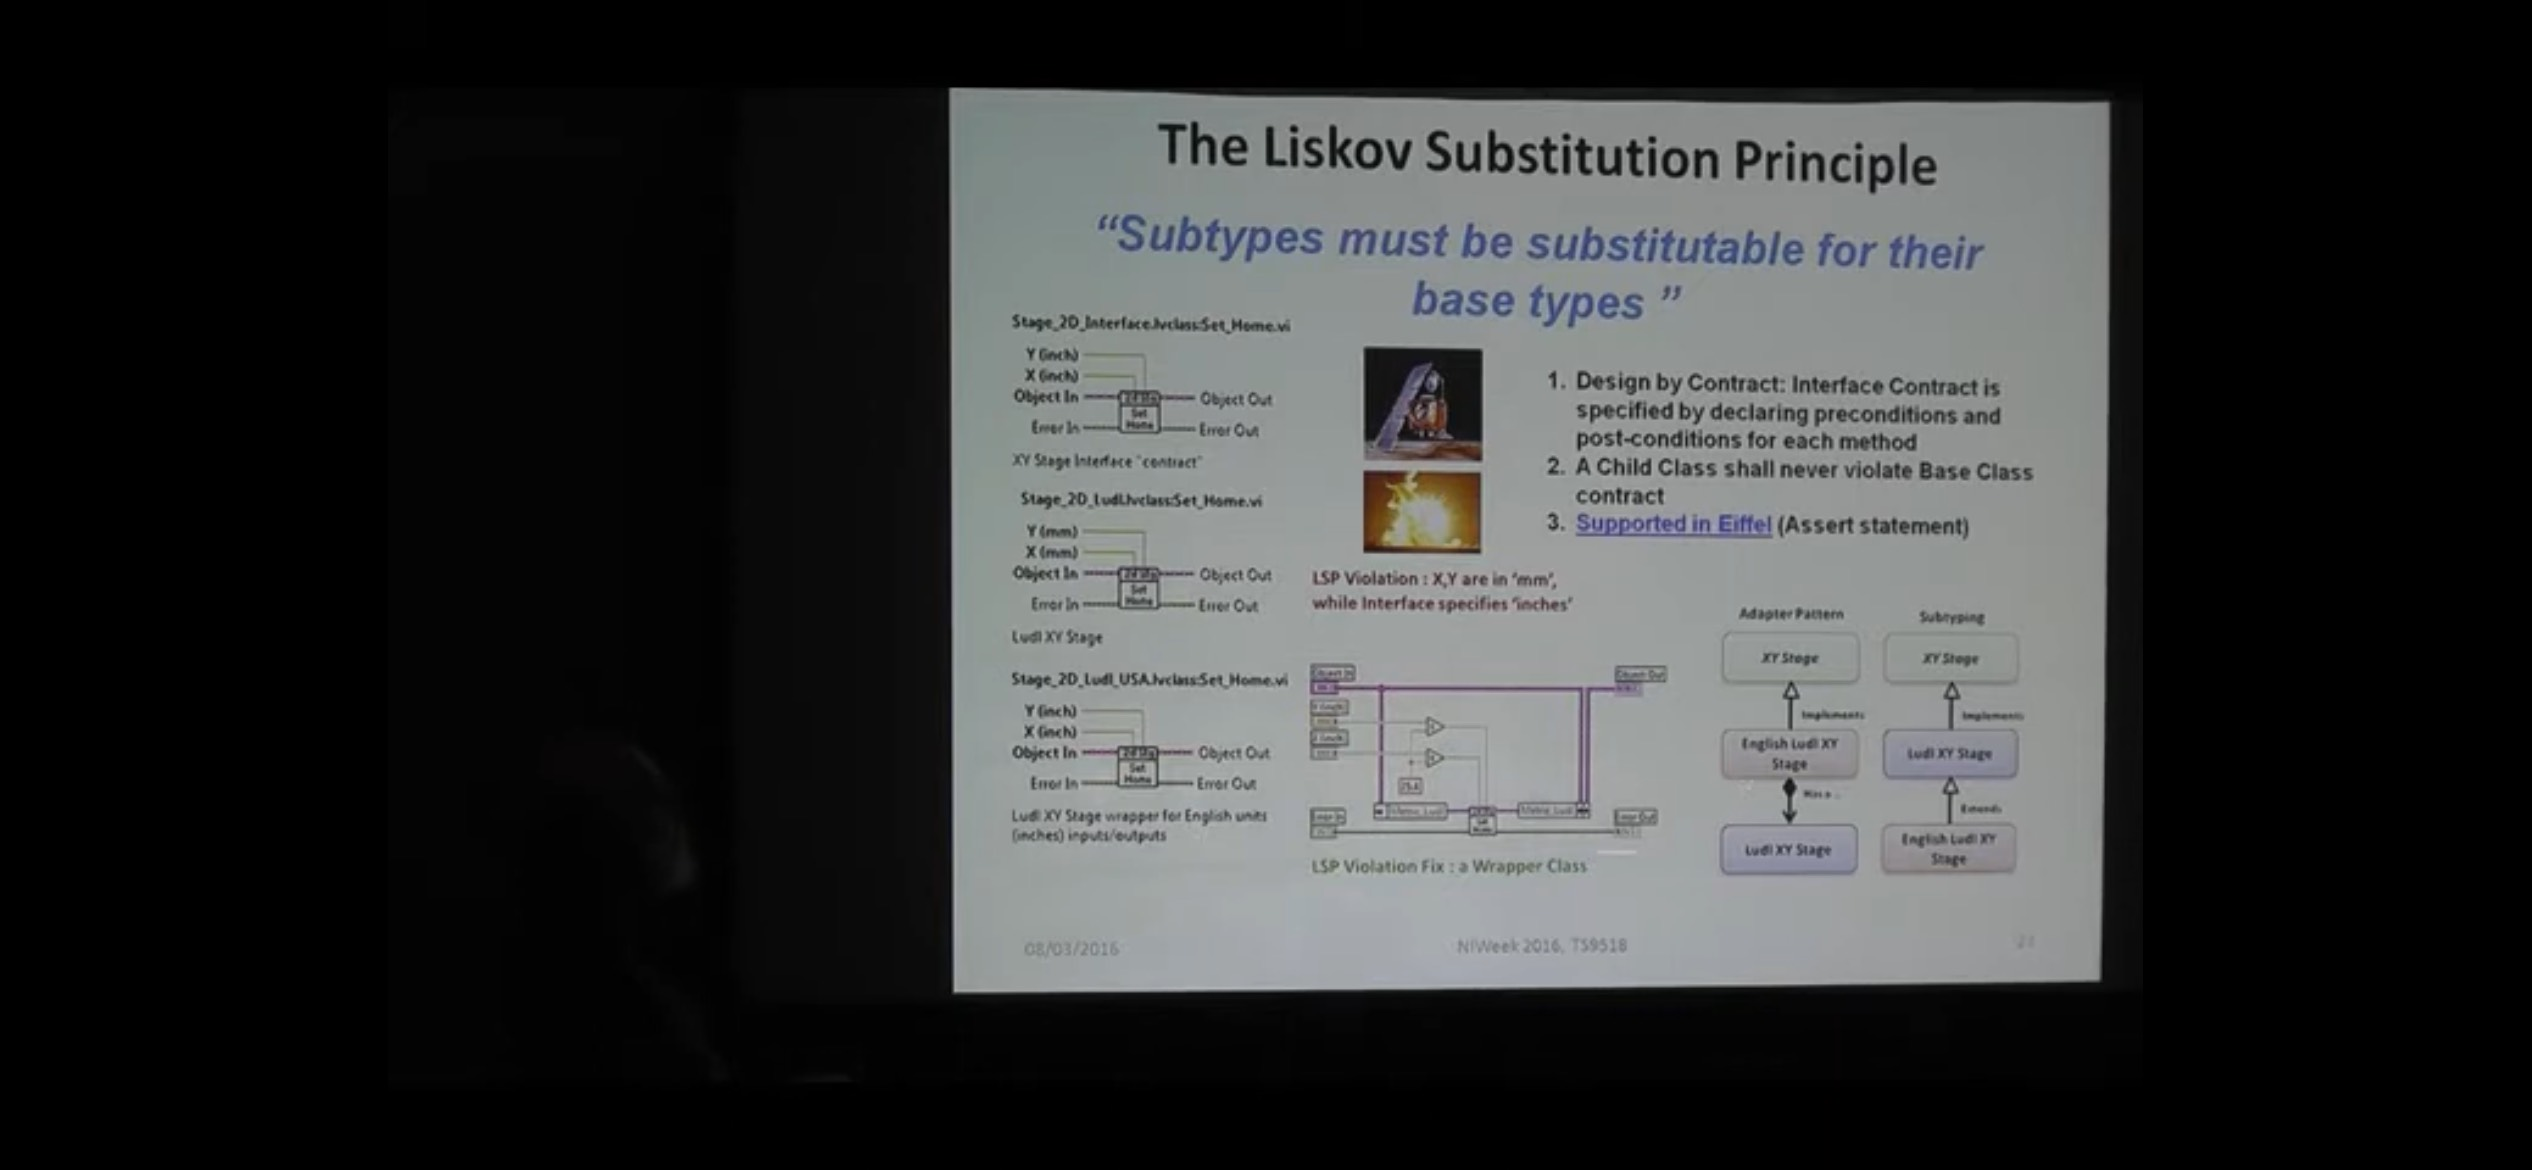
\includegraphics[width=0.8\textwidth]{figures/dmitry_liskov_sub_principle}
    \caption{This image shows the naming convention for LabVIEW classes and methods.}
    \label{fig:dmitry-liskov-sub-principle}
\end{figure}

Noting that Fig~\ref{fig:dmitry-liskov-sub-principle} shows the naming convention for LabVIEW classes and methods.
\begin{itemize}
    \item{Library-Name.lvlib}
    \item{Interface-Name.lvclass}
    \item{Class-Name.lvclass (control is capital by default!)}
    \item{method-Name.vi}
    \item{control-Name.ctl (this control, which is not tied to a class is lowercase!)}
\end{itemize}

\noindent Note: Avoid underscores and spaces.

\section{Design Patterns}
\label{sec:design-patterns}

\subsection{State Pattern}
\label{subsec:state-pattern}

\noindent Context:

\quad Method.vi (just a wrapper for Method.vi “State”).\footnote{Best Practice: use this Method.vi in other methods, rather than the Method.vi “State” itself}

\noindent State.lvclass (interface):

\quad Concrete State.lvclass

\quad Method.vi “State”

\section{External Packages}
\label{sec:external-packages}

\href{https://www.vipm.io/package/illuminatedg_lib_ig_oopanel/}{IG OOPanel}

\subsection{Panels}
\label{subsec:panels}

Actor helpers, not helper actors.
Helper Loop → Async Actor Helper.
These are helper loops that are created async which help an actor with its task.
This is to declutter the actor by offloading certain tasks such as panel display or subprocesses that do not require an additional actor to be created.

\subsection{UI Events}
\label{subsec:ui-events}

Indicators: Instead of generating an event, bundle in the reference of the indicator and have a property node (write)in the subVI.

The same can be said for the control, which has a right click menu, that bundles in the reference for the control and creates a subVI that writes the value to the front panel.
Or creates a signal, something that automatically puts the control in the event loop and bundles in the reference for the control to the subVI.
Create control which does the same as the indicators but added the reference of the control to the private data.

In prelaunch, have a subVI that internally has the creation of the user events.
Script to create the subVI first.

Interface with DD methods:
No need for template to replace the placeholder methods with new ones, just have DD methods as “placeholders” which change their implementation depending on the class that's on the wire

\begin{figure}[!ht]
    \centering
    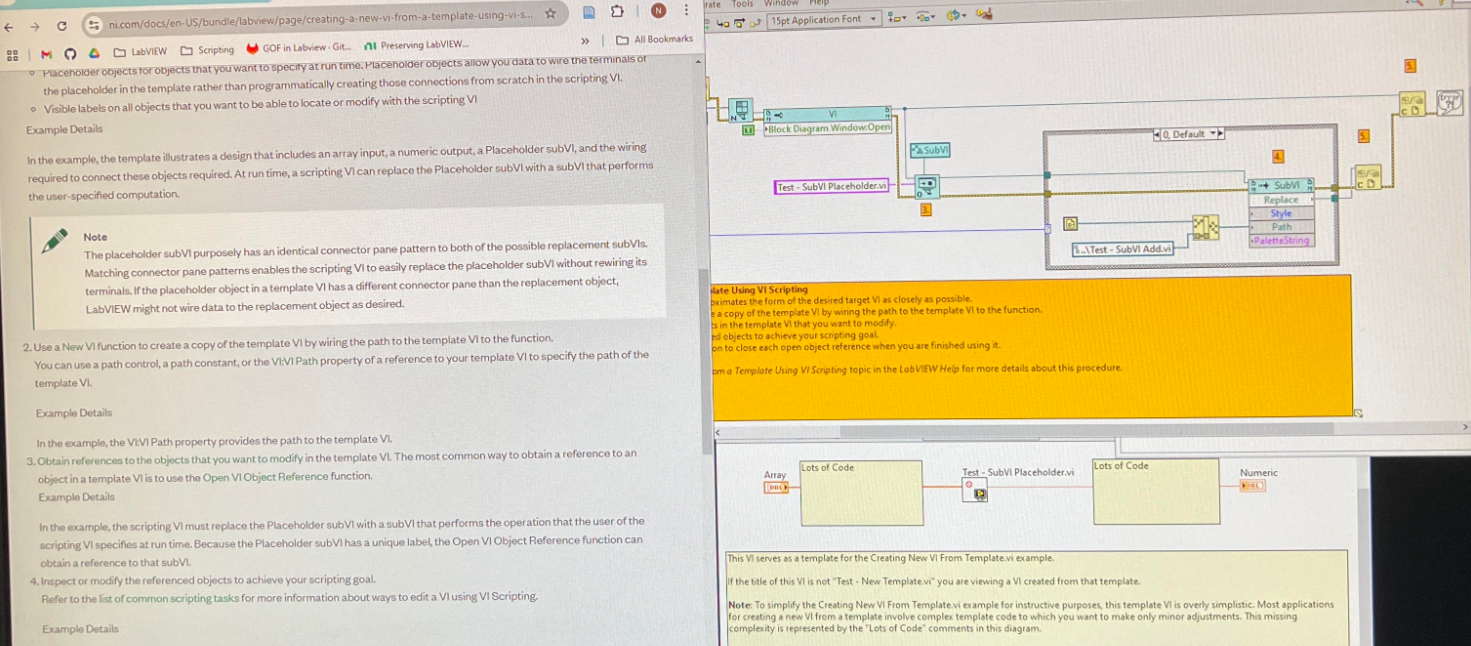
\includegraphics[width=0.8\textwidth]{figures/justACS_ui_events}
    \caption{This image shows the UI events in LabVIEW.}
    \label{fig:justacs-ui-events}
\end{figure}

Split the events as controls and indicators as shown in Fig~\ref{fig:justacs-ui-events}.

\subsection{Right Click creates library with interface}

Method in actor: \\
Creates library containing interface and method along with message class with Send and Do methods

\section{Messaging}
\label{sec:messaging}

Actor messages error on generation of message.
Error when creating a message and wiring in the interface object as an input, the message scripting doesn't know how to differentiate the class input and the parameter input


\section{Scripting}
\label{sec:scripting}

Go through and replace all the Opens and Traverse with the hidden gem.

User groups for the scripting (quick drop, right click, etc.).


\section{TODO}
\label{sec:todo}

Non-reentrant methods → shared reentrant

Have the interface checkbox for DD methods not required for override doesn't necessarily break subtype rules!

In the DD methods, because they are not required to be overridden, have functionality within them that calls the Self Actor method (some kind of checking mechanism?).

Actor interface methods (all implemented with default functionality) to have the *new* (Actor Interface) Read Actor DD method that reads from the Dev Actor the Self Actor class and performs that interface function, then bundles back in with the Setup method.

Do this for all for the default behavior.

Note this is breaking the contract for interface DD methods not needing to be overridden.

Instead of the Setup method, create a new Actor Write method which ONLY Writes to the Actor. This can also be put inside the Setup method as a first step, the setup code follows after

State Enter Core and State Exit Core are NOT check marked.
That way the developer does not need to override, just to have no functionality anyway.
Read State and Write State do because they'll have functionality.

\section{Miscellaneous}
\label{sec:miscellaneous}

\subsection{MEF (Managed Extensibility Framework)}
\label{subsec:mef}

\href{https://www.youtube.com/watch?v=rrtz7sKCg2A}{LabVIEW Interfaces for Satellite Calibration - SLM and McBee}: 44:50

\section{Errors}
\label{sec:errors}

In frameworks, errors are fundamental to the program's operation. They are not just incidental issues but rather integral to the design and flow of the application.
jettl has an error object in the private data of the jettl object. At the end of the method, the error object is unbundled and checked for errors before teardown.

\begin{figure}[h]
    \centering
    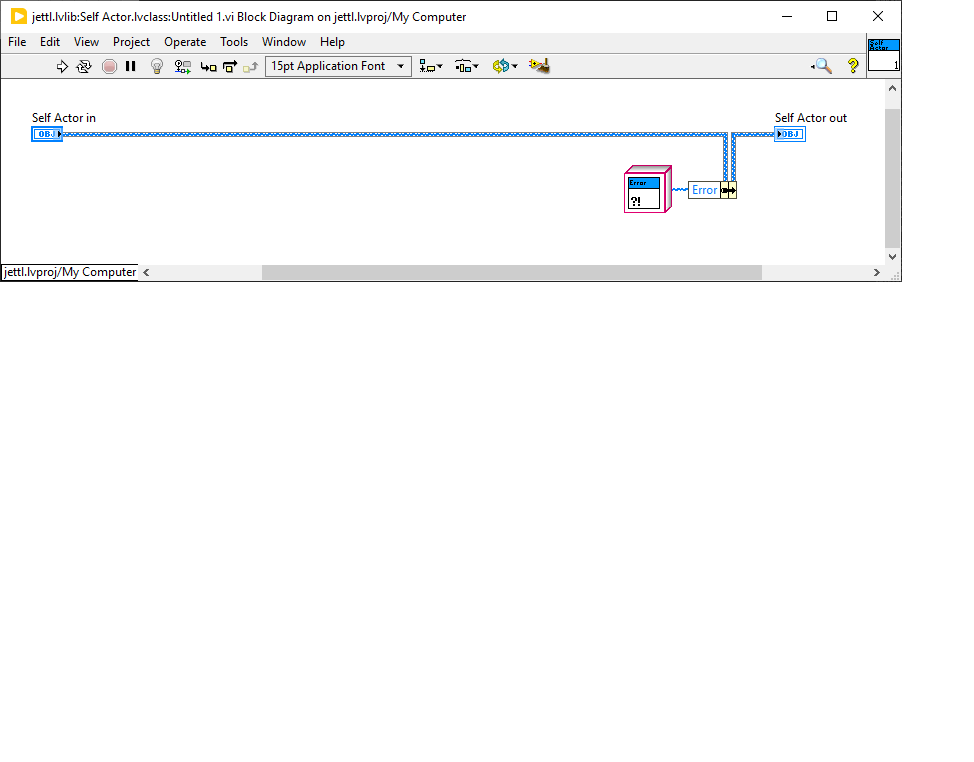
\includegraphics[width=0.8\textwidth]{figures/method-template}
    \caption{Method template. This has no error terminals, and the error object is handled internally. This is a different approach to error handling in LabVIEW methods.}
    \label{fig:method-template}
\end{figure}

Wouldn't this make the API more beautiful and easy to understand? Having just the object wire come out of the method, and ONLY the object wire coming out of the method?
I suppose, adopting the OO paradigm.
Instead of having the error cluster inside the objects class data.
Instead, it's a dedicated “error object” shared for every single object in use.
Encourages data flow since unbundling of errors will always occur.
It's a step in the right direction having no “error input” for methods.
Now it's time to get rid of the error out.
It's almost like branching an objects wire, in a way. There should only be one thing coming out of a method.

\end{document}
